\chapter{Task \#15: Cascading Failures - SOC model }
\section{Introduction}

\textbf{Self-Organized Criticality} (SOC) is an approach adopted to explain the emergence of power-law distributions in natural phenomena. 
In physics, criticality is associated to systems near phase transitions, that live between two distinct regimes, 
and at this critical point, the emergence of power-laws occurs.

\noindent In SOC, systems are believed to organize themselves naturally into critical states, following internal feedback mechanisms and without external intervention.


\noindent In this report, we analyze the SOC behavior associated to the Sandpile Model.

\noindent In the \textbf{Sandpile Model}, we consider networks with an associated load variable, that accounts for any sort of stress that can be observed in real applications. 
A given node in the network stays functional, as long as its load doesn't go above a given threshold: its \textit{capacity}. 
Load is assigned randomly to nodes in the network, and when the capacity of a node is overcome, we have a failure in the node, and its load is redistributed according to some chosen rules. 
A dissipative factor is added to load transfers, to avoid excessive accumulation of load across the network.

\noindent We use single-layer\footnote{ Following the works \cite{doi:10.1143/JPSJ.64.327} and \cite{PhysRevLett.91.148701}.} and two-layer\footnote{ Following \cite{doi:10.1073/pnas.1110586109}.} synthetic networks, where the first ones are used to examine the basic properties of cascade failures, 
and the second offers a more robust study of interconnected systems, such as real power grids.

\noindent To analyze the cascades, we assume a tree structure of each avalanche, and using the theory of multiplicative branching processes, 
we find analytical predictions for the distributions of the size of the avalanches $p(s)$ and of their lifetime $l(t)$.


\noindent Considering:
\begin{gather}
    p(s)\sim s^{-\tau}
    \\
    l(t)\sim t^{-z}
\end{gather}
The results for the single layer systems studied in this work are reported in Tab.~\ref{tab:analytical_res}. 
For interconnected networks, the analytical results for each single layer are not obtained, but considering the distributions of cascades over the whole network, 
the results are equivalent to a random network.

\begin{table}[htbp]
    \centering
    \begin{tabular}{lc|c|c}
        \toprule
        \textbf{Network} && $\tau$ & $z$ \\
        \midrule
        Random && $3/2$ & $2$ \\
        \hline
        & $2<\gamma<3$ & $\frac{\gamma}{\gamma-1}$ & $\frac{\gamma-1}{\gamma-2}$ \\
        Scale-free ($\gamma$) & $\gamma=3$ & $3/2^*$ & $2^*$\\
        & $\gamma\ge3$ & $3/2$ & $2$\\
        \bottomrule
    \end{tabular}
    \caption{Analytical predictions for avalanche distributions. \\
    $^*$ with logarithmic corrections.}
    \label{tab:analytical_res}
\end{table}

\noindent  

\section{Sandpile Model on Single Layer Networks} 

\noindent We first consider the Sandpile Model on single layer networks with simple degree distributions, in particular, following the works of Bonabeau \cite{doi:10.1143/JPSJ.64.327} and Goh \emph{et al.}~\cite{PhysRevLett.91.148701}, we use the distributions:
\begin{itemize}  
    \item Gaussian (Random): $k \sim \mathcal{N}(\mu=20,\sigma=8)$
    \item Uniform (Random): $k\sim\text{Uniform}(k_{\mathrm{min}}=4,k_{\mathrm{max}}=36)$
    \item Power Law (Scale Free): $k\sim k^{-\gamma}$ with $\gamma\in\{2.01,2.2,2.4,2.6,2.8,3.0,5.0\}$
\end{itemize}

\noindent Every network includes $N=10^5$ nodes, and the results are the averages of $30$ different iterations.
The dissipation is carried by dissipative nodes ($0.1\%$ of the total) in the random networks, which transfer load outside of the network once toppled; we use a dissipation probability $f=0.001$ on the scale-free network, 
which is the probability of every load transfer to not happen, dissipating the load.


\noindent Fig.~\ref{fig:part1} displays the results obtained for avalanche size and lifetime distributions in the random networks. 
Excluding dissipation effects, visible on the heads of the distributions, and finite-size effects, visible on their tails, 
the results follow the analytical prediction, shown in the dashed line.

\begin{figure}[htbp]
    \centering
    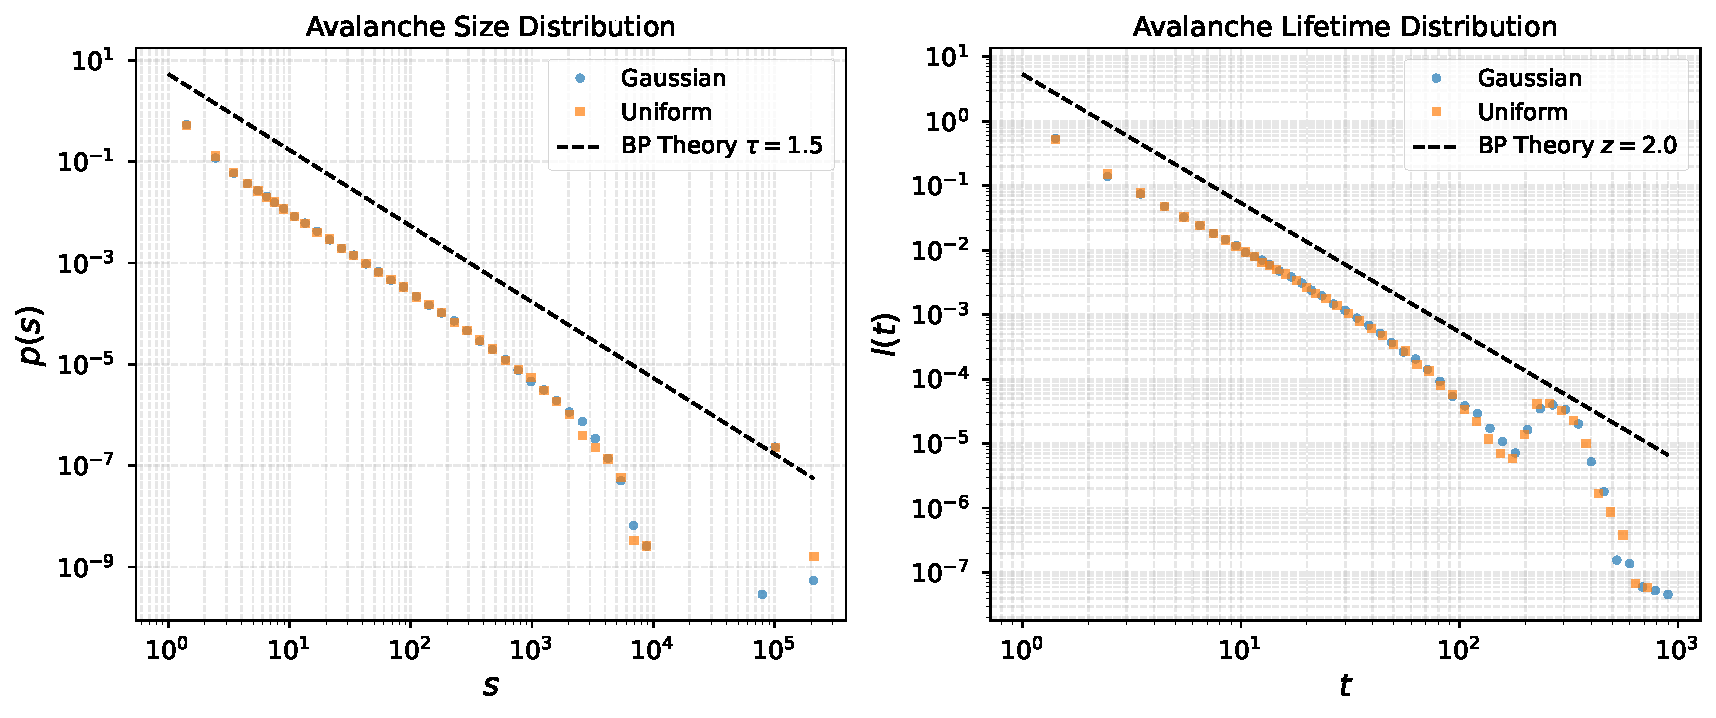
\includegraphics[width=0.9\textwidth]{./figures/task_15/task_15_part1.pdf}
    \caption{Avalanche size ($s$) and lifetime ($t$) distributions for the sandpile model on Gaussian and Uniform networks, along with the expected theoretical results (dashed lines).}
    \label{fig:part1}
\end{figure}

\noindent The results for the scale-free networks are reported in Section~\ref{sec:appendix1}, along with a brief analysis on the exponents extracted from the distributions.   
\section{Interconnected Networks}

\noindent We conclude the analysis by studying how interconnectivity between two networks affects cascading failures, following the work of Brummitt \emph{et al.}~\cite{doi:10.1073/pnas.1110586109}. 
Real power grids are sparsely interconnected with narrow degree distributions; to model this we consider two independent random 3-regular graphs, each with $N=2\times10^3$ nodes, coupled by a \emph{Bernoulli interconnection}: each node of either network independently receives one additional external edge stub with probability $p$ (and none with probability $1-p$). 
The external stubs of the two networks are then matched uniformly at random, so that both networks have the same number of interconnections. 
We denote this topology by $R(3)\text{-}B(p)\text{-}R(3)$; the threshold of each node is its total degree, as before.

\noindent We run the sandpile dynamics with dissipation rate $f=0.01$, chosen so that the largest cascades topple almost the entire network, dropping $2\times10^6$ grains per realization (after a $20\%$ transient) on $30$ independent realizations for $10$ values of $p$ in $[0.001,\,0.5]$, concentrating on small $p$ as in the reference work.


\noindent We define $T_o$ as the number of topplings caused in network $o\in\{a,b\}$, and $T_{m,n}$ as the number of topplings in network $n$ caused by a cascade started in network $m$.

\begin{figure}[htbp]
    \centering
    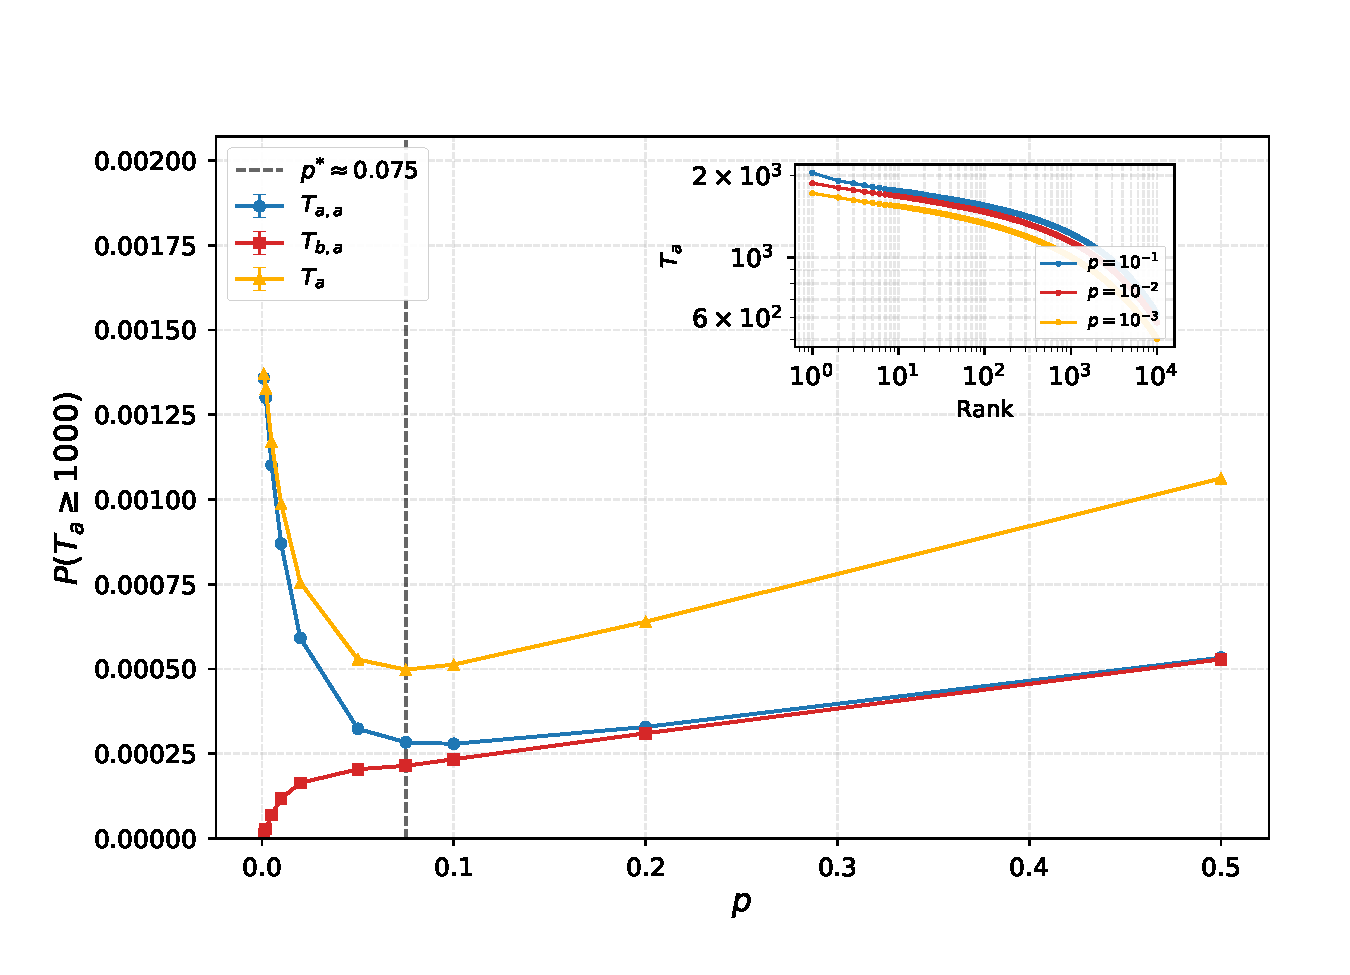
\includegraphics[width=0.85\textwidth]{./figures/task_15/task_15_part3_fig4.pdf}
    \caption{Probability of a large avalanche ($T_a>1000=N/2$) in network $a$ as a function of the interconnectivity $p$.
    Large cascades \emph{beginning} in $a$ (blue) first decrease and then increase with $p$, whereas cascades beginning in $b$ and toppling most of $a$ (red) become monotonically more likely.
    Large cascades in $a$ are minimized at $p^{*}\approx0.075$.
    Inset: log-log rank-size plots of the $10^4$ largest values of $T_a$ for $p=10^{-1},10^{-2},10^{-3}$, showing the suppression of the largest local cascades as interconnectivity is initially increased.}
    \label{fig:part3_fig4}
\end{figure}

\noindent Figure~\ref{fig:part3_fig4} shows the central result: adding a few interconnections between the networks is \emph{locally stabilizing}, the probability of a large avalanche in $a$ ($T_a>N/2$) initially drops with $p$, because excess load is absorbed by the neighboring network, which acts as a reservoir.
However, beyond a critical amount of interconnectivity the probability rises again, for two reasons: interconnections open pathways for network $b$ to inflict large cascades onto $a$ (the red curve only ever increases), and every added interconnection augments the total capacity and average load of the system, fueling larger cascades.
The two effects balance at $p^{*}\approx0.075$, where the probability of a large avalanche in $a$ is minimized.


\noindent The effects of increased connectivity on global stability and different avalanche sizes are investigated in Section~\ref{sec:appendix1}.

\newpage

\section{Supplementary Material}\label{sec:appendix1}

\subsection{Scale-Free Networks}
Fig.~\ref{fig:part2} displays the avalanche size and lifetime distributions for the scale-free networks, at the chosen gamma values. The results follow the theoretical predictions for $\gamma \geq 3$. 

\begin{figure}[htbp]
    \centering
    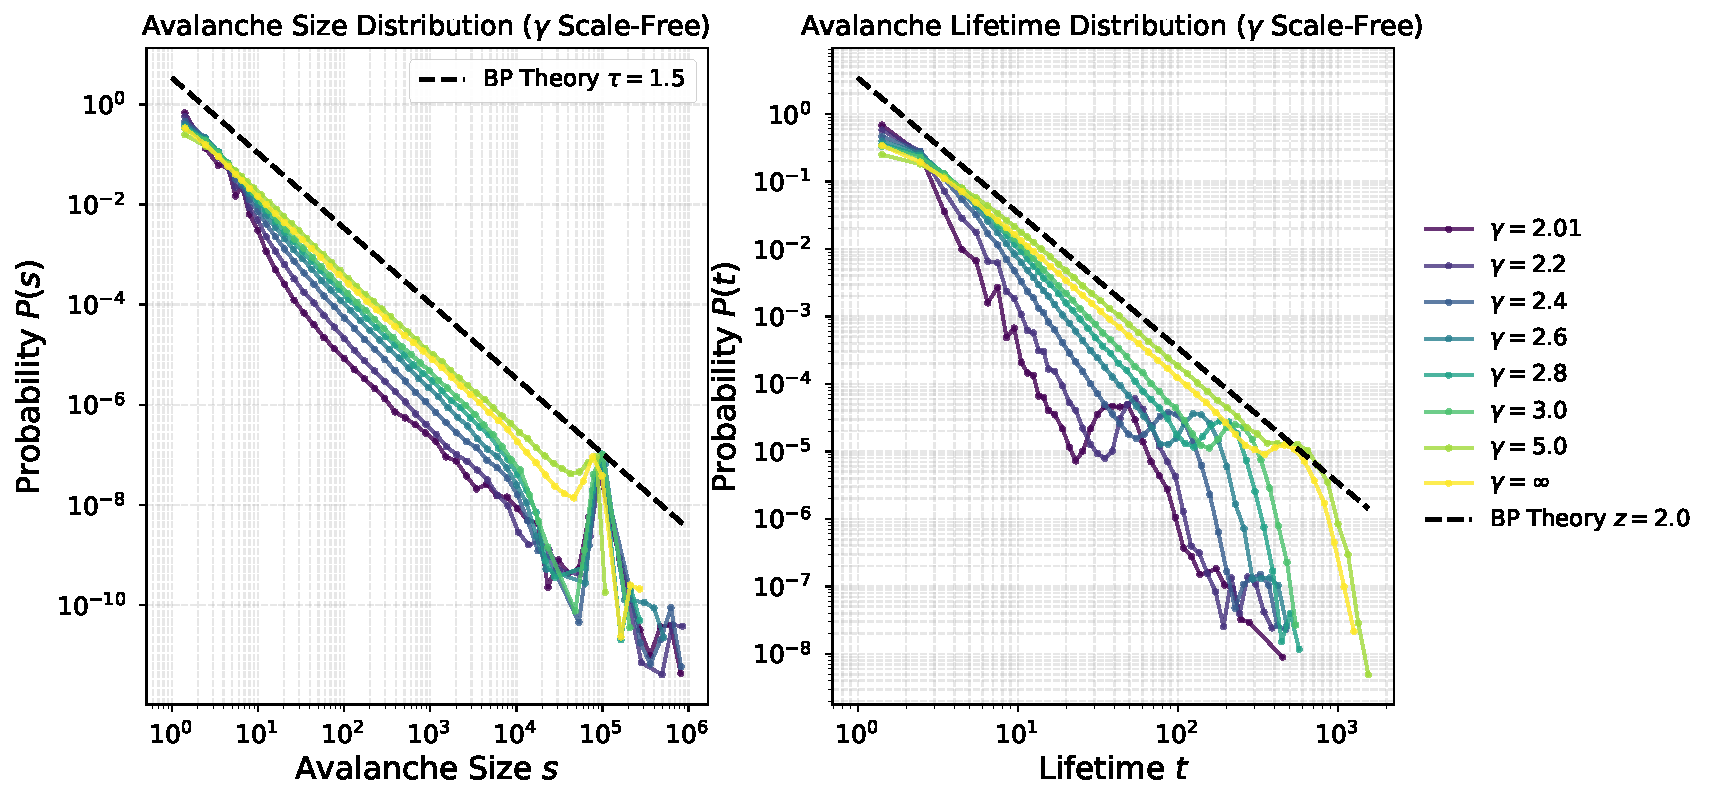
\includegraphics[width=0.9\textwidth]{./figures/task_15/task_15_part2.pdf}
    \caption{Avalanche size ($s$) and lifetime ($t$) distributions for the sandpile model on Scale-Free networks, 
    along with the expected theoretical results for $\gamma \geq 3$ (dashed lines).}
    \label{fig:part2}
\end{figure}

\subsection{Exponents Analysis}
To analyze other gamma values, we estimate the scaling exponents fitting the observed distributions, and report the results in Tab.~\ref{tab:fitted_exponents}. 


\noindent For each distribution the fitting window is chosen as the longest straight window: sliding a lower cutoff over a set of candidates and the upper edge is extended as far as the weighted least-squares fit maintains a coefficient of determination\footnote{$R^2=1-\frac{SS_{res}}{SS_{tot}}$, where $SS_{res} =\sum_i(y_i-f(x_i))^2$ is the squared residuals between data $y_i$ and predictions $f(x_i)$; and $SS_{tot}=\sum_i(y_i-\bar{y})^2$ is a coefficient proportional to the variance of the dataset. }
$R^2\ge0.999$ for the avalanche sizes and $R^2\ge0.998$ for the (noisier) lifetimes. Finally, the window with the largest logarithmic span is selected. The window chosen for each fit is reported in the Table.

\noindent The error bars in the exponents are the standard deviation of the exponent over the family of plausible windows obtained by varying the $R^2$ threshold and the lower cutoff by one step. 
This systematic uncertainty, reflecting how much the exponent changes under a relocation of the fitting window, dominates the scatter of the regressions.

\begin{table}[htbp]
    \centering
    \resizebox{\textwidth}{!}{%
    \begin{tabular}{lc|cc|cc|cc|cc}
        \toprule
        \textbf{Network} && \multicolumn{2}{c|}{$\tau$} & \multicolumn{2}{c|}{$z$} & \multicolumn{2}{c|}{$s$} & \multicolumn{2}{c}{$t$} \\
        & & theory & fit & theory & fit & min & max & min & max \\
        \midrule
        Gaussian && 1.50 & 1.62 $\pm$ 0.01 & 2.00 & 1.98 $\pm$ 0.06 & 5 & 3e+03 & 4 & 6e+01 \\
        Uniform && 1.50 & 1.61 $\pm$ 0.01 & 2.00 & 2.00 $\pm$ 0.05 & 5 & 3e+03 & 4 & 6e+01 \\
        $\gamma = 2.01$ && 1.99 & 1.75 $\pm$ 0.10 & 101.00 & 5.58 $\pm$ 0.21 & 58 & 4e+02 & 54 & 1e+02 \\
        $\gamma = 2.2$ && 1.83 & 1.81 $\pm$ 0.06 & 6.00 & 5.90 $\pm$ 0.33 & 58 & 3e+03 & 68 & 2e+02 \\
        $\gamma = 2.4$ && 1.71 & 1.76 $\pm$ 0.03 & 3.50 & 3.44 $\pm$ 0.05 & 58 & 1e+04 & 6 & 6e+01 \\
        $\gamma = 2.6$ && 1.62 & 1.79 $\pm$ 0.04 & 2.67 & 2.90 $\pm$ 0.03 & 20 & 1e+04 & 4 & 1e+02 \\
        $\gamma = 2.8$ && 1.56 & 1.75 $\pm$ 0.02 & 2.25 & 2.62 $\pm$ 0.04 & 20 & 6e+04 & 4 & 1e+02 \\
        $\gamma = 3.0$ && 1.50 & 1.72 $\pm$ 0.03 & 2.00 & 2.42 $\pm$ 0.03 & 17 & 2e+04 & 4 & 2e+02 \\
        $\gamma = 5.0$ && 1.50 & 1.60 $\pm$ 0.00 & 2.00 & 1.95 $\pm$ 0.09 & 5 & 3e+04 & 4 & 7e+02 \\
        $\gamma = \infty$ && 1.50 & 1.63 $\pm$ 0.01 & 2.00 & 2.03 $\pm$ 0.02 & 5 & 6e+04 & 4 & 5e+02 \\
        \bottomrule
    \end{tabular}}
    \caption{Fitted avalanche-size ($\tau$) and lifetime ($z$) exponents vs multiplicative branching-process predictions, together with the scaling ranges used for each fit.
    Fits are performed on the longest straight window of each log-binned distribution and
    error bars are the window-sensitivity of the fit (see text). 
    The corresponding fit windows are listed, $s$ refers to size intervals and $t$ to lifetime intervals.}
    \label{tab:fitted_exponents}
\end{table}

\noindent The fitted exponents are in good agreement with the multiplicative branching process predictions: 
on the random networks the lifetime exponent matches $z = 2$ within the window-sensitivity error, and the size exponent sits only slightly above the mean-field value $\tau = 3/2$ (a finite-size effect visible in the mild slope drift of the local slopes). 
For the scale-free networks the observed exponents decrease with $\gamma$ as predicted, although the fitted $\tau$ remains below the theoretical value for $\gamma = 2.01$ and rises above it for $\gamma \gtrsim 2.4$; 
for $\gamma$ close to $2$ the theoretical lifetime exponent diverges as $z = (\gamma-1)/(\gamma-2)$, which is not attainable in finite networks, so the comparison there is only indicative.

\subsection{Interconnected Networks}
\begin{figure}[htbp]
    \centering
    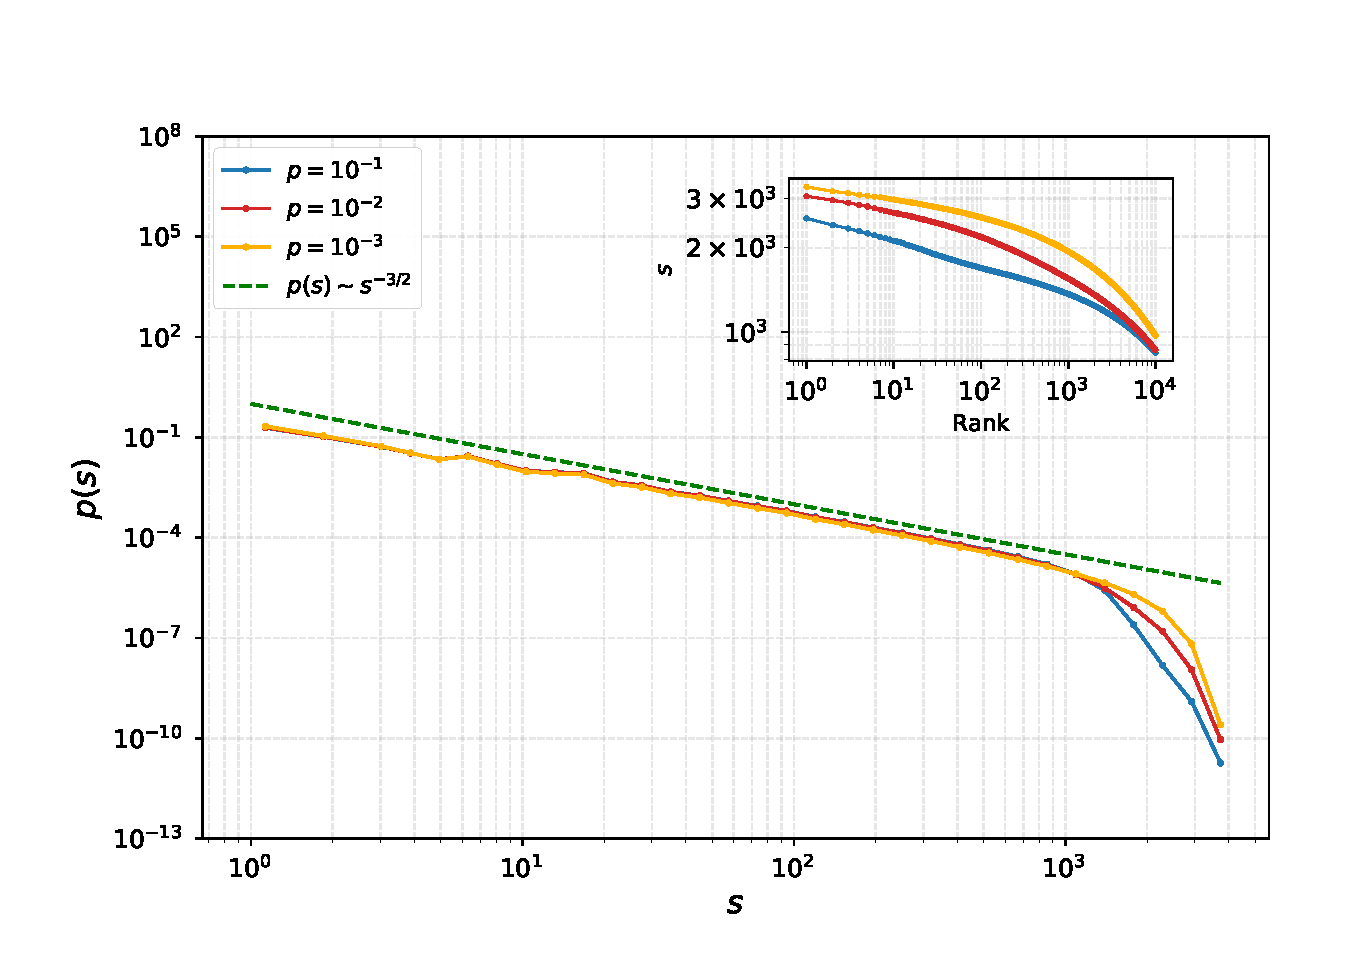
\includegraphics[width=0.85\textwidth]{./figures/task_15/task_15_part3_fig5.pdf}
    \caption{Total avalanche size distribution $p(s)$ (topplings in both networks) on $R(3)\text{-}B(p)\text{-}R(3)$ for $p=10^{-3},10^{-2},10^{-1}$, in log-log.
    The green dashed line is the mean-field prediction $p(s)\sim s^{-3/2}$ obtained when both networks are viewed as a single system.
    Inset: log-log rank-size plot of the $10^4$ largest global cascades, showing that increasing $p$ enlarges the largest cascades of the whole system due to the additional interconnections.}
    \label{fig:part3_fig5}
\end{figure}

\noindent The locally stabilizing effect is specific to each individual network; the collection of networks viewed as one system is instead \emph{globally destabilized} by interconnectivity.
Figure~\ref{fig:part3_fig5} shows that the total avalanche size distribution $p(s)$ (considering topplings in both networks) develops a longer tail as $p$ grows, 
and the inset confirms that the largest global cascades become larger with $p$: while a single network benefits from interconnectivity, the whole system suffers larger cascades.

\begin{figure}[htbp]
    \centering
    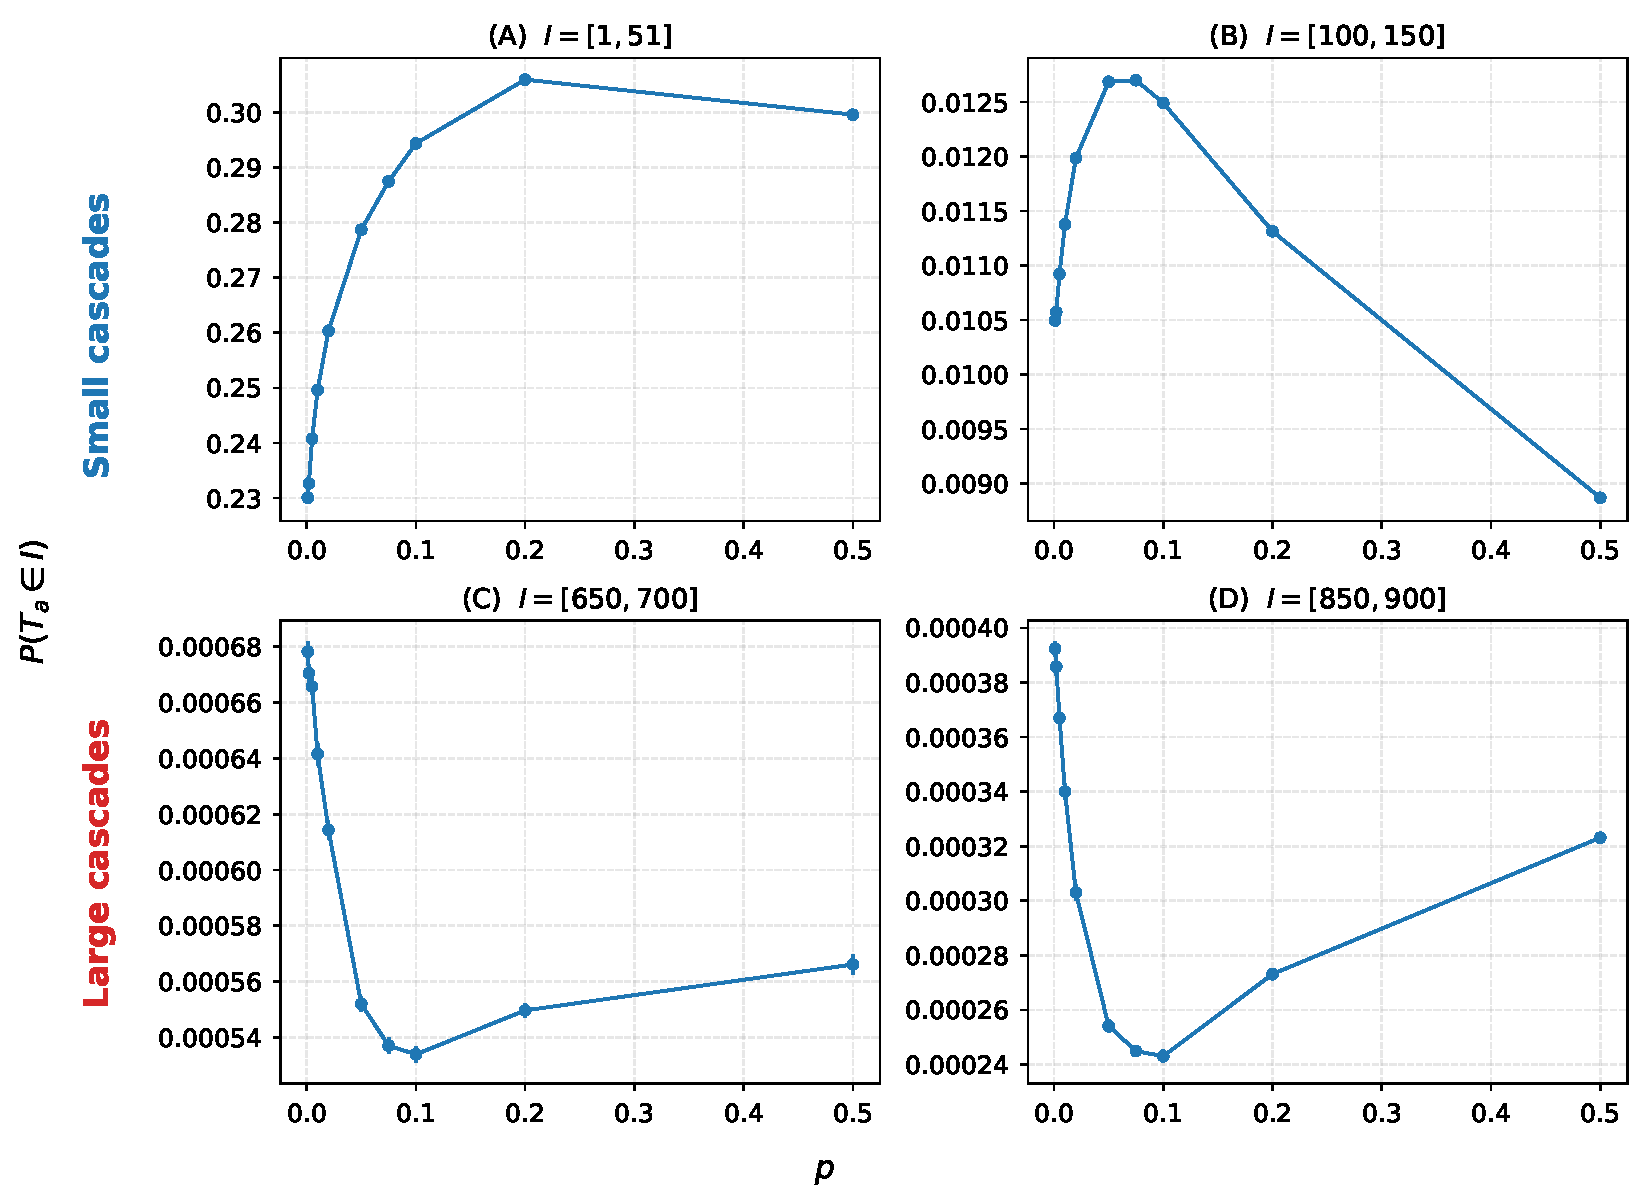
\includegraphics[width=0.85\textwidth]{./figures/task_15/task_15_part3_fig6.pdf}
    \caption{Probability that a cascade in network $a$ has total size $T_a$ within each of four windows, as a function of $p$ on $R(3)\text{-}B(p)\text{-}R(3)$.
    Small cascades (A) become more likely with $p$; intermediate cascades (B) peak at an unstable critical point near $p^{*}\approx0.075$; the largest cascades (C, D) are minimized at the stable equilibrium $p^{*}\approx0.075$.
    Tuning the interconnectivity to suppress one range of cascade sizes amplifies the others.}
    \label{fig:part3_fig6}
\end{figure}

\noindent Figure~\ref{fig:part3_fig6} shows that the effect of interconnectivity depends on the size of the cascade considered: small cascades ($1\le T_a\le51$) are favored by larger $p$, intermediate cascades ($100\le T_a\le150$) occur most frequently at an unstable critical point around $p^{*}\approx0.075$, while the largest cascades ($650\le T_a\le700$ and $850\le T_a\le900$) are suppressed at the same equilibrium point $p^{*}$.
A network cannot simultaneously mitigate all cascade sizes: interconnectivity that minimizes the largest cascades amplifies the intermediate ones, and vice versa.
